%%%%%%%%%%%%%%%%%%%
% SECTION: Regulatization
%%%%%%%%%%%%%%%%%%%
\subsection{Regularization Techniques}

Deep architectures usually have millions of parameters, each layer is connected by weight connections. 
Many of these relationships can become really complicated, which are the result of sampling noise. These models with a lot of parameters can easily overfit the training data. Much of the noise exists in the training set but not in test or real data even if they are drawn from the same distribution. To help avoid this problem, there exist regularization methods that have been developed to help reduce it.

% SECTION: Dropout
\subsubsection{Dropout}
Dropout is a technique that prevents overfitting. The term refers to dropping out units in a neural network. Dropping units mean that they will be remove from the network, including the inputs and outputs connections. Dropout uses a fixed probability $p$ to be retained. The choice of units to be dropped is random \cite{Srivastava2014Dropout:Overfitting}.

% FIGURE: dropout
\begin{figure}[H]	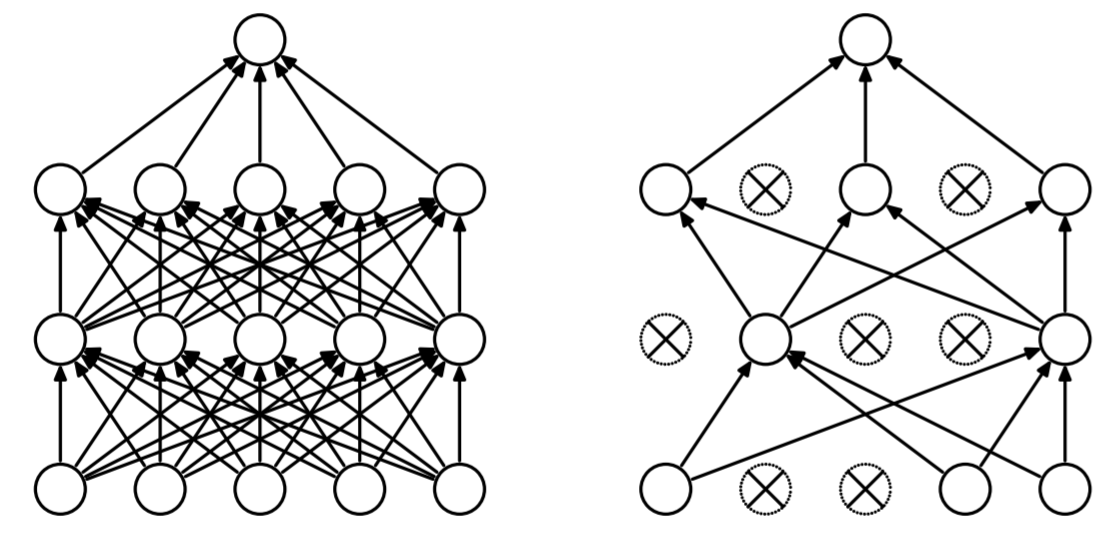
\includegraphics[width=0.8\textwidth]{images/dropout.png} 
    \centering

\caption{Left: A standard neural net with 2 hidden layers. Right: An example of a thinned net produced by applying dropout to the network on the left. \cite{Srivastava2014Dropout:Overfitting} } 

\label{fig:dropout}
\end{figure}

% SECTION: L1/L2 Regularization
\subsubsection{L1/L2 Regularization}
L1 and L2 regularization adds a term that prevents the coefficient to fit perfectly to the data, thus preventing overfitting. L1, equation \ref{eq:l1}, is the sum of the weights. 

\begin{equation} \label{eq:l1}
w^{*}= arg \underset{w}{min} \sum_{j} \left ( t(x_{j})- \sum_{i}w_{i}h_{i}(x_{j}) \right )^{2} + \lambda \sum_{i=1}^{k}\left | w_{i} \right |
\end{equation}

The L2 regularization in equation \ref{eq:l2}, is the sum of the square of the weights.

\begin{equation} \label{eq:l2}
w^{*}= arg \underset{w}{min} \sum_{j} \left ( t(x_{j})- \sum_{i}w_{i}h_{i}(x_{j}) \right )^{2} + \lambda \sum_{i=1}^{k} w_{i}^{2}
\end{equation}

http://www.chioka.in/differences-between-l1-and-l2-as-loss-function-and-regularization/

% SECTION: Batch Normalization
\subsubsection{Batch Normalization}
This regularization technique normalizes the input batch using the mean and variance. Batch normalization solves problems related to weight initialization; and also normalization speeds up convergence, even when the features are not decorrelated. Normalization is performed for each mini-batch by propagating the gradients through the normalization parameters. Batch Normalization adds two extra parameters per activation. Even with these parameters, it is able to preserve the representation ability of the network. \cite{Choromanska2015BatchShift}